\chapter{Überblick}

Die Gesamtaufgabe wurde in mehrere Subaufgaben geteilt, damit jeder Schritt einzeln bearbeitet und analysiert werden kann. Somit wird gewährleistet, dass die Übersichtlichkeit auch bei größeren Schaltungen nicht verloren geht. Sollte jedoch trotz der Aufteilung in kleinere Teilschritte ein Problem auftreten, kann dank der Überschaubarkeit schnell und effizient der Fehler gefunden und behoben werden. \smallskip \smallskip

\begin{figure}[htbp]
	\centering
	\fbox{
		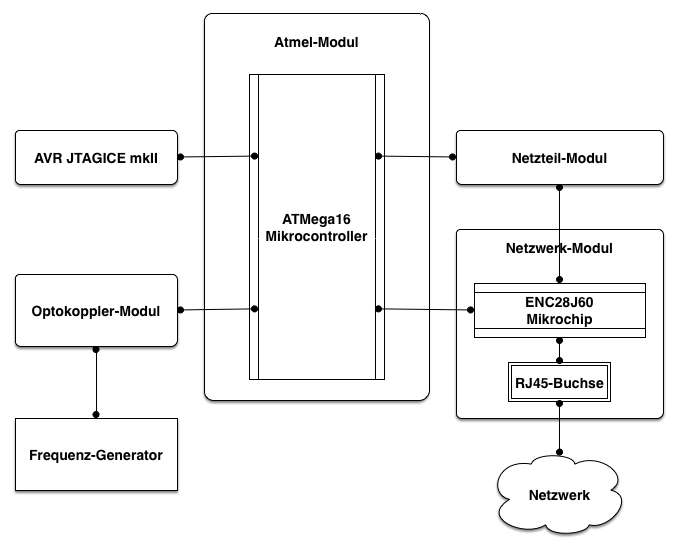
\includegraphics[width=310px,height=250px]{pictures/entwurf.png}
	}
	\caption{Zusammenbau von allen Modulen}\label{fig:aufbau}
\end{figure}

Die \autoref{fig:aufbau} zeigt, wie die einzelnen Module im Gesamtsystem miteinander verbunden sind. Danach wurde der Schaltplan laut dem obigen Gesamtsystem im Eagle\footnote{ist ein Program der Firma CadSoft zur Erstellung von Leiterplatte zur Entwurfsautomatisierung elektronischer Systeme.}-Schaltplaneditor \cite{Cadsoft:Eagle} erstellt. Die Gesamtschaltung ist im \autoref{anhang:schaltung} zu sehen. \smallskip \smallskip

Es wird eine Schnittstelle, sog. \textbf{AVR JTAGICE mkII}, zwischen dem Atmel-Modul und dem verwendeten Rechner angeschlossen. Dieses Modul ermöglicht die Programmierung des ATmega16-Mikrocontrollers. \smallskip \smallskip

Das \textbf{Optokoppler-Modul} liest ein kontinuierlich-sinusförmiges Signal aus dem Frequenzgenerator aus und digitalisiert dieses Signal. Anschließend wird das kontinuerlich-digitalisierte Signal an den Eingangspin des Atmel-Moduls weitergeleitet. \smallskip \smallskip

Das \textbf{Atmel-Modul} liest das Eingangssignal aus dem Pin und sogleich beschäftigt es sich mit der Abarbeitung der Frequenzmessung des Signals mittels eines internen Timers. Nachfolgend werden die Messungswerte dem Netzwerk-Modul abgegeben, wenn sie abgefragt werden. \smallskip \smallskip

Das \textbf{Netzwerk-Modul} ist eine Kommunikationsschnittstelle für das UDP-Protokoll zwischen dem Atmel-Modul und einem beliebigen UNIX-Server. Die Frequenzwerten werden nach Anforderung des Servers über das Netzwerk-Modul weitergegeben. Für die Abfrage wird ein Dämon zum Laufen auf UNIX basierten Systemen programmiert. \smallskip \smallskip

Jedes Modul des Gesamtsystems wird im nächsten Kapitel näher beschrieben. Im \autoref{chapter:protokoll} wurde das Kommunikationsprotokoll näher unter die Lupe genommen. Außerdem ist im \autoref{anhang:software} auch das programmierte Kommunikationsprotokoll zu lesen.

